\documentclass[12pt]{article}

\usepackage{german}
\usepackage{geometry}
\usepackage[onehalfspacing]{setspace}

\geometry{
    left=3cm,
    right=3cm,
    top=2.5cm,
    bottom=2.5cm
}

\usepackage{listings}
\usepackage{xcolor}

\usepackage{amsmath}
\usepackage{amssymb}

\usepackage{url}

\usepackage{tikz}

\setlength{\emergencystretch}{15pt}

\lstset{
    tabsize = 4, %% set tab space width
    showstringspaces = false, %% prevent space marking in strings, string is defined as the text that is generally printed directly to the console
    numbers = left, %% display line numbers on the left
    commentstyle = \color{green}, %% set comment color
    keywordstyle = \color{blue}, %% set keyword color
    stringstyle = \color{red}, %% set string color
    rulecolor = \color{black}, %% set frame color to avoid being affected by text color
    basicstyle = \small \ttfamily , %% set listing font and size
    breaklines = true, %% enable line breaking
    numberstyle = \tiny,
}

\title{Numerisches finden von Nullstellen - Implementierung in Java}
\author{Jakob Rzeppa}

\begin{document}
\begin{titlepage}
	\centering
    {\huge IGSFF LOGO TODO\par}
	{Grünewaldstraße 12a - 38104 Braunschweig - T. 470 5850\par}
	\vspace{1cm}
	{\underline{Seminarfach:}\par}
	\vspace{1cm}
    {\large Facharbeit des Schülers \textit{Jakob Rzeppa} \par mit dem Thema: \par}
    \vspace{1.5cm}
	{\huge Numerisches finden von Nullstellen - Implementierung in Java\par}
	\vspace{2cm}
\end{titlepage}

\tableofcontents

\section{Einleitung}

\subsection{Problemstellung}

\subsection{Verwendungszwecke}

\section{Weierstraß-Iteration}
Die Weierstraß-Iteration, auch genannt Durand-Kerner-Methode, ist ein iteratives Verfahren, zur numerischen Bestimmung aller komplexen Nullstellen einer univariaten\footnote{Univariat bedeutet, dass eine Funktion nur eine Variable hat.} Polynomfunktion.
Sie wurde von Karl Weierstraß zwischen 1859 und 1891 als Teil seines Beweises des Fundamentalsatzes der Algebra entwickelt und 1960 von Durand sowie 1966 von Immo Kerner unabhängig voneinander wiederentwickelt.
Die Weierstraß-Iteration findet die Nullstellen im Gegensatz zum Newton-Horner-Verfahren\footnote{
    Das Newton-Horner-Verfahren ist eine Kombination der Newton-Methode und des Horner-Schemas. Dabei wird eine Nullstelle mithilfe der Newton-Methode gefunden und dannach mithilfe des Horner-Schemas von der Funktion entfernt. Das Verfahren wird bis alle Nullstellen gefunden wurden wiederholt.
}
nicht nacheinander, sondern parallel. Das bedeutet, dass bei jedem Schritt jede Nullstelle genauer wird und nicht jede Nullstelle nacheinander approximiert wird.\footnote{
    vgl. Wikipedia: Durand-Kerner method, URL: \url{https://en.wikipedia.org/wiki/Durand-Kerner_method} (Zuletzt eingesehen am 29.10.2023)
    \label{ftn:Wikipedia-Durand-Kerner-Method}
}

%----------------------------------------------------------------------------------------------------
\section{Funktionsweise}
\subsection{Bedingungen}
Für die Weierstraß-Iteration muss ein normiertes univariates Polynom der Form $p(x) = x^n + a_{n-1} x^{n-1} + \dots + a_1 x + a_0$ gegeben sein. Der Grad $n$ des Polynoms muss größer als zwei sein.\footnote{
    vgl. Wikipedia: Weierstraß-(Durand-Kerner)-Verfahren, URL: \url{https://de.wikipedia.org/wiki/Weierstraß-(Durand-Kerner)-Verfahren} (Zuletzt eingesehen am 29.10.2023)
    \label{ftn:Wikipedia-Weierstraß-Methode}
}

\subsection{Fixpunktiteration der Weierstraß-Iteration}
Bei der Weierstraß-Iteration wird mit jeder Iteration jede Nullstelle etwas genauer. Dafür werden $n$ Gleichungen für die $n$ Nullstellen\footnote{Eine Funktion $n$ten Grades hat nach dem Fundamentalsatz der Algebra genau $n$ komplexe Nullstellen.} $z_n;z_{n-1};\dots;z_1$ gebildet. Über diese wird, bis das Endkriterium erreicht ist, iteriert. Dabei ist $i$ die Anzahl der Iterationen und wird pro Iteration um 1 inkrementiert.
\[z_n^{(i+1)} = z_n^{(i)} - \frac{p(z_n^{(i)})}{\prod_{j=1;j\neq n}^{n}(z_n^{(i)}-z_j^{(i)})}\]
\[z_{n-1}^{(i+1)} = z_{n-1}^{(i)} - \frac{p(z_{n-1}^{(i)})}{\prod_{j=1;j\neq n-1}^{n}(z_{n-1}^{(i)}-z_j^{(i)})}\]
\vspace{0.25mm}
\[\dots\]
\[z_{1}^{(i+1)} = z_1^{(i)} - \frac{p(z_{1}^{(i)})}{\prod_{j=1;j\neq 1}^{n}(z_{1}^{(i)}-z_j^{(i)})}\]
\subsection{Startpunkte}
Zunächst müssen alle Startpunkte $z_n^{(0)};z_{n-1}^{(0)};\dots;z_1^{(0)} \in \mathbb{C}$ gesetzt werden. Diese können beliebig gewählt werden. Es muss jedoch beachtet werden, dass Startpunkte für komplexe Nullstellen einen imaginären Teil ungleich Null haben. Außerdem müssen alle Startpunkte unterschiedlich sein, damit bei der ersten Iteration nicht durch Null dividiert wird.
Denn bei der Gleichung
\begin{equation*}
    z_k^{(i+1)} = \frac{p(z_{k}^{(i)})}{\prod_{j=1;j\neq k}^{n}(z_{k}^{(i)}-z_j^{(i)})}
\end{equation*}
wird, wenn $z_{k}^{(i)}$ gleich einem anderen $z^{(i)}$ ist, durch Null dividiert.
Die Startpunkte können allerdings auch die Anzahl der Iterationen beeinflussen. Deswegen macht es Sinn, möglichst nahe an den wahrscheinlichen Nullstellen anzufangen.\\
Eine der gängigsten Methoden ist, die Startpunkte in einem Kreis auf der komplexen Ebene zu verteilen. Dabei ist der Radius $r = \sqrt[n]{|a_0|}$ relativ genau. Jedoch ist es sehr ressourcenintensiv Wurzeln zu berechnen. Deshalb kann auch ein weniger genauerer Radius genommen werden: $r = |\frac{na_0}{2a_1}| + |\frac{a_{n-1}}{2n}|$.
Auf dem Kreis werden alle Startpunkte gleichmäßig verteilt, indem der Kreis in $n$ Abschnitte geteilt wird, an dessen Anfängen die Startpunkte liegen. Dafür wird das Inkrement $\theta = \frac{2\pi}{n} \text{ bzw. } \frac{360^\circ}{n}$ benötigt. Zuletzt wird noch eine Verschiebung $c$ durchgeführt, um keine reellen Startpunkte zu erhalten. Diese kann beliebig gewählt werden, solange keine reellen Zahlen nach der Verschiebung unter den Startpunkten sind. Bei der folgenden Implementierung wurde $c = \frac{\pi}{2n}$ gewählt.
Um die Startpunkte zu bestimmen wird 
\[z_{k}^{(0)} = r\cos((k-1)\theta+c)+r\sin((k-1)\theta+c)i \text{ für } k=1;2;\dots;n\]
angewand.\footnote{
    vgl. Oscar Veliz: Durand-Kerner Method: Minute 5:40 (Veröffentlicht am 29.05.2019), URL: \url{https://www.youtube.com/watch?v=5JcpOj2KtWc} (Zuletzt eingesehen am 30.10.2023) \label{ftn:OscarVilez,5:40}
}

\subsection{Endkriterium}
Um zu bestimmen, ob eine Nullstelle gefunden wurde, muss eine gewünschte Genauigkeit $g$ (z.B. $0,0001$) gewählt werden. Diese wird dann mit dem Betrag der Differenz der letzten beiden Schritten der Weierstraß-Iteration verglichen. Ist $|z_k^{(i-1)}-z_k^{(i)}| < g$ wahr ist die Nullstelle $z_k$ auf die Genauigkeit $g$ gefunden. Dies wird für alle Nullstellen wiederholt. Falls alle Nullstellen genau genug sind ist die Weierstraß-Iteration abgeschlossen.\\
Es kann jedoch auch vorkommen, dass die Weierstraß-Iteration nicht konvergiert. Darauf wird in dem Abschnitt Probleme und Einschränkungen noch eingegangen. Allerdings muss deswegen eine weitere Endbedingung gestellt sein: eine maximale Anzahl an Iterationen. Dabei muss man wissen, mit welchen Polynomen man zutun hat. Sind diese sehr komplex kann es vorkommen, dass die Weierstraß-Iteration weit über Tausend Iterationen benötigt, um eine vernünftige Genauigkeit zu geben. In solchen Fällen muss man das Limit sehr hoch setzen. In meiner Implementierung wurde ein Limit von 1000 gesetzt um für die meist vorkommenden Polynome zuverlässig zu funktionieren.

%-----------------------------------------------------------------------------------------------------------
\section{Beispiel}
Im Folgenden wird die Weierstraß-Iteration an einer Polynomfunktion vierten Grades beispielhaft durchgeführt. Dabei wird die Genauigkeit im Beispiel auf vier Nachkommastellen begrenzt, was zu Ungenauigkeiten kleiner als $0,0001$ führen kann.
\paragraph{Fixpunktiteration der Weierstraß-Iteration}
Für die Funktion
\begin{equation*}
    p(x) = x^4 + 4x^3 - 2x^2 + 3x - 4 = (x-z_1)(x-z_2)(x-z_3)(x-z_4)
\end{equation*}
sind die Nullstellen $z_1;z_2;z_3;z_4 \in \mathbb{C}$ gesucht. Für jede der Nullstellen wird, wie zuvor beschrieben, eine Gleichung gebildet:
\begin{equation*}
    z_1^{(i+1)} = z_1^{(i)}-\frac{p(z_1^{(i)})}{(z_1^{(i)}-z_2^{(i)})(z_1^{(i)}-z_3^{(i)})(z_1^{(i)}-z_4^{(i)})}
\end{equation*}
\begin{equation*}
    z_2^{(i+1)} = z_2^{(i)}-\frac{p(z_2^{(i)})}{(z_2^{(i)}-z_1^{(i)})(z_2^{(i)}-z_3^{(i)})(z_2^{(i)}-z_4^{(i)})}
\end{equation*}
\begin{equation*}
    z_3^{(i+1)} = z_3^{(i)}-\frac{p(z_3^{(i)})}{(z_3^{(i)}-z_1^{(i)})(z_3^{(i)}-z_2^{(i)})(z_3^{(i)}-z_4^{(i)})}
\end{equation*}
\begin{equation*}
    z_4^{(i+1)} = z_4^{(i)}-\frac{p(z_4^{(i)})}{(z_4^{(i)}-z_1^{(i)})(z_4^{(i)}-z_2^{(i)})(z_4^{(i)}-z_3^{(i)})}
\end{equation*}
\paragraph{Startpunkte}
Zuvor müssen allerdings die Startpunkte $z_1^{(0)};z_2^{(0)};z_3^{(0)};z_4^{(0)}$ bestimmt werden. Dabei ist der Radius des Kreises $r = |\frac{na_0}{2a_1}| + |\frac{a_{n-1}}{2na_n}| = \frac{19}{6}$, der Abstand zwischen den Startpunkten $\theta = \frac{2\pi}{n} = \frac{1}{2}\pi$ und die Verschiebung $c = \frac{\pi}{2n} = \frac{1}{8}\pi$. Mit diesen Werten können die Startpunkte berechnet werden. \\
$z_1^{(0)} = r \cos(c) + r \sin(c)i = 2,9256 + 1,2118i$ \\
$z_2^{(0)} = r \cos(\theta+c) + r \sin(\theta+c)i = -1,2118 + 2,9256i$ \\
$z_3^{(0)} = r \cos(2\theta+c) + r \sin(2\theta+c)i = -2,9256 - 1,2118i$ \\
$z_4^{(0)} = r \cos(3\theta+c) + r \sin(3\theta+c)i = 1,2118 - 2,9256i$

\paragraph{Ausführung}
\begin{center}
\begin{tabular}{c|c c c c}
    Iteration & $z_1$ & $z_3$ & $z_2$ & $z_4$ \\
    \hline
    0 & 2,9256 + 1,2118i & -1,2118 + 2,9256i & -2,9256 - 1,2118i & 1,2118 - 2,9256i \\
    1 & 1,2993 + 0,8722i & -1,8873 + 2,0075i & -3,405 - 0,7665i & -0,0069 - 2,1133i \\
    2 & 1,0806 + 0,5889i & -1,1784 + 0,4767i & -4,1287 + 0,3433i & 0,2265 - 1,4089 \\
    3 & 0,7884 + 0,3817i & -0,2138 + 0,7292i & -4,6806 - 0,0989 & 0,1061 - 1,012i \\
    4 & 0,6759 - 0,234i & 0,0243 + 0,9804i & -4,613 - 0,0021i & -0,0872 - 0,9549i \\
    5 & 0,8621 + 0,0197i & -0,1294 + 0,9945i & -4,6149 & -0,1177 - 1,0141i \\
    6 & 0,842 + 0,0004i & -0,1134 + 1,0078i & -4,6149 & -0,1136 - 1,0082i \\
    7 & 0,8421 & -0,1136 + 1,0081i & -4,6149 & -0,1136 - 1,0081i \\
    8 & 0,8421 & -0,1136 + 1,0081i & -4,6149 & -0,1136 - 1,0081i \\
\end{tabular}
\end{center}
\paragraph{Endkriterium}
Zwischen Iteration Sieben und Acht ist die Differenz zwischen den beiden Werten für jede Nullstelle kleiner als die Genauigkeit $0,0001$. Damit ist das Endkriterium erreicht und die Weierstraß-Iteration abgeschlossen. 
Die Nullstellen der Polynomfunktion $p(x) = x^4 + 4x^3 - 2x^2 + 3x - 4$ sind bei ca. $0,8421; -4,6149; -0,1136 - 1,0081i; -0,1136 + 1,0081$. 
\paragraph{Probe}
Zur Überpfüfung kann jeder der Werte in $p(x)$ eingesetzt werden.
\begin{displaymath}
    f(0,8421) \approx 0; p(-4,6149) \approx 0; f(-0,1136 - 1,0081i) \approx 0; p(-0,1136 + 1,0081i) \approx 0
\end{displaymath}
Daraus kann geschlossen werden, dass alle vier Werte Annährungen der Nullstellen der Polynomfunktion $p(x)$ sind. \\
Weiterhin, kann aus dem Fundermentalsatz der Algebra hergeleitet werden, dass alle Nullstellen von $p(x)$ gefunden wurden, da $n$ gleich der Anzahl der gefunden Nullstellen ist. \\
$\Rightarrow$ Die Weierstraß-Iteration war für $p(x)$ erfolgreich.

\section{Visualisierung}
TODO (maybe bei Beispiel)


%--------------------------------------------------------------
\section{Herleitung}
In diesem Abschnitt wird auf die Herleitung der Methode und der bestimmung der Startpunkte eingegangen.
\subsection{Methode}
Im Folgenden wird, um es verständlicher zu machen, die Herleitung der Methode nur mit reellen Zahlen durchgeführt. Jedoch kann dies ohne Probleme auf komplexe Zahlen übertragen werden.
\paragraph{Visualisierung}
Für die Herleitung der Methode macht es Sinn den Graph einer einzelnen Gleichung mit immer genaueren restlichen Nullstellen zu visualisieren. Dabei ist $z_k^{(i)} = x$ und $z_k^{(i+1)} = y$:
\begin{equation}
    g(x) = y = x - \frac{p(x)}{\prod_{j=1;j\neq k}^{n} (x-z_j^{(i)})}
\end{equation}
\begin{figure}[h]
    \centering
    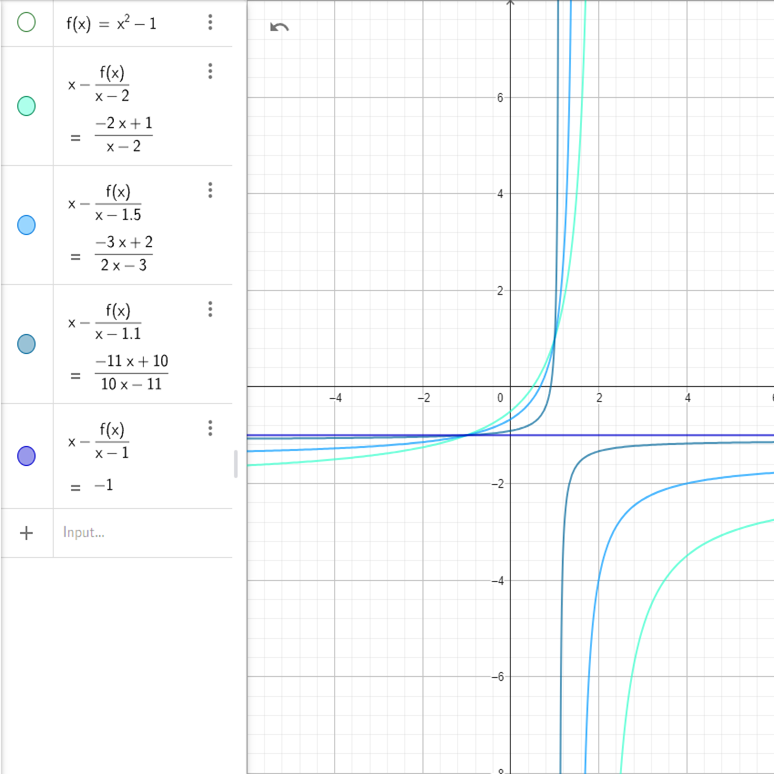
\includegraphics[scale=.6]{BeispielHerleitung.png}
    \caption{Beispiel: $x^2-1$ für die Nullstelle $-1$}
    %TODO
\end{figure}\\
%-------------------------------------------------------------------------------------------------------------------
Dabei sieht man, dass es sich, wenn die restlichen Nullstellen nicht genau sind, um eine gebrochen rationale Funktion\footnote{Das kann auch an der Gleichung selber gesehen werden, da diese, mit ein wenig umstellen, aus einem Polynom geteilt durch ein anderes Polynom besteht.} handelt und wenn die restlichen Nullstellen gefunden wurden um eine waagrechte lineare Funktion\footnote{Das liegt daran, dass alle linearen Faktoren des Polynoms, außer dem der gesuchten Nullstelle, gefunden wurden und nun von dem Polynom abgezogen werden. Dabei bleibt $x-(x+z_k^{(i)})$ über. Die beiden $x$ fallen weg und es bleibt ein konstanter Wert über. Daraus folgt, dass die Funktion waagrecht zu der x-Achse ist.}. 
%-------------------------------------------------------------------------------------------------------------------
\paragraph{Waagrechte Asymptote}
Hat waagrechte Asymptote
Sieht man daran:
\begin{align*}
    y &= x - \frac{p(x)}{\prod_{j=1;j\neq k}^{n} (x-z_j^{(i)})} \\
    &= \frac{x}{1} - \frac{\prod_{j=1}^{n} (x-z_j^{(i)})}{\prod_{j=1;j\neq k}^{n} (x-z_j^{(i)})} \\
    &= \frac{x \cdot \prod_{j=1;j\neq k}^{n} (x-z_j^{(i)})}{\prod_{j=1;j\neq k}^{n} (x-z_j^{(i)})} - \frac{\prod_{j=1}^{n} (x-z_j^{(i)})}{\prod_{j=1;j\neq k}^{n} (x-z_j^{(i)})} \\
    &= \frac{x \cdot \prod_{j=1;j\neq k}^{n} (x-z_j^{(i)}) - \prod_{j=1}^{n} (x-z_j^{(i)})}{\prod_{j=1;j\neq k}^{n} (x-z_j^{(i)})} \\
\end{align*}
Da die Polynome im Zähler normiert und vom gleichen Grad sind kann, besitzen beide den Term $a_nx^n$ mit $a_n = 1$. Werden diese Polynome nun miteinander subtrahiert, fällt der $n$te-Term weg, da dieser bei beiden Polynomen gleich ist. Somit ist der Grad des Differenzpolynoms $n-1$. \\
\begin{equation*}
    y = \frac{\text{Polynom vom Grad }n-1}{\text{Polynom vom Grad }n-1}
\end{equation*}
%-------------------------------------------------------------------------------------------------------------------
\paragraph{Bedeuteung für die Weierstraß-Iteration}
Mit der ersten Iteration wird, falls weit genug von Definitionslücke weg, auf positive oder negative seite gegangen
    Beweis, dass waagrechte Asymptote gleiches vorzeichen wie nullstelle hat
\\
Da waagrechte Asymptote -> Mit nötigem Abstand zu Definitionslücken $|g(x)|<|x|$
-> Methode \glqq entkommt\grqq\space nicht
-> geht, Mit nötigem Abstand zu Definitionslücken $|g(x)|<|x|$, näher an die Nullstelle herran
%-------------------------------------------------------------------------------------------------------------------
\paragraph{verhalten in der nähe der Nullstelle}
$g(x)$ wird immer genauer, wenn die anderen Nullstellen genauer werden
-> alles wird genauer parallel
%-------------------------------------------------------------------------------------------------------------------
\paragraph{verhalten auf der Nullstelle}
$g(z_k) = z_k$ -> Konvergiert -> Nullstelle gefundne
\\
Kann man auch daran sehen:
\begin{align*}
    y &= x - \frac{p(x)}{\prod_{j=1;j\neq k}^{n} (x-z_j)} \\
    &= x - (x-z_k) \\
    &= z_k
\end{align*}
%-------------------------------------------------------------------------------------------------------------------
\paragraph{Außnahmen und Probleme}
Wenn zu nah an Definitionslücke verfälschte Werte
Kann ein Sprung weg sein -> verfälschung aller Werte -> mehr Iterationen benötigt
\\
Manchmal nicht Konvergiert, weil hin und herspringen von nähe von Definitionslücken

\subsection{Wählen der Startpunkte}
Alle Nullstellen einer Polynomfunktion befinden sich auf der abgeschlossen Kreisscheibe  $B(0,M) := \{x \in \mathbb{C} \bigr| |x| \le M\}$ mit $M := 1 + \max\{\frac{|a_j|}{|a_n|}\bigr|\text{\space}j=0,\dots,n-1\}$.\footnote{vgl. \glqq\textit{Sei $P(z) = a_nz^n+a_{n-1}z^{n-1}+\dots+a_1z+a_0$ ein komplexes Polynom vom Grad $n \ge 1$. Dann liegen alle Nullstellen von $P(z)$ in der abgeschlossenen Kreisscheibe $B(0,M) := \{z \in \mathbb{C} \bigr| |z| \le M\}$, wobei $M := 1 + \max\{\frac{|a_j|}{|a_n|}\bigr|\text{\space}j=0,\dots,n-1\}$.}\grqq\space Humboldt-Universität zu Berlin: Helga Baum: Nullstellen komplexer Polynome: 6.3. Erster Satz von Cauchy, URL: \url{https://didaktik.mathematik.hu-berlin.de/user/fehlingerl/Helga.pdf} (Zuletzt eingesehen am 30.10.2023)}  Um möglichst genaue Startpunkte zu bekommen kann man diese auf einer Kreislinie innerhalb der Kreisscheibe anordnen. \\
Dabei gibt es keinen \glqq besten\grqq\space Standart für das Wählen des Radius. Jeder Radius ist für manche Funktionen näher und andere weiter von den Nullstellen entfernt. Je nach den Anforderungen kann man einen eigenen Radius für die Kreislinie nehmen. In meiner Implementierung habe ich mich deshalb für $r = |\frac{na_0}{2a_1}| + |\frac{a_{n-1}}{2n}|$ entschieden.\footref{ftn:OscarVilez,5:40}
Dieser Radius ist relativ ressourcensparend und einfach zu implementieren. Jedoch kann auch ein anderer Radius gewählt werden.

%------------------------------------------------------------------------------------
\section{Probleme und Einschränkungen}
Die Weierstraß-Iteration hat, neben dem Vorteil, dass sie einfach zu implementieren ist mehrere Nachteile. Auf diese wird im Folgenden eingegangen.
\subsection{Normiertes Polynom}
Für die Weierstraß-Iteration muss die gegebene Funktion $p(x)$ in der Form $\prod_{i=1}^n (x-z_i)$ dargestellt werden können. Da $\prod_{i=1}^n (x-z_i)$ ausmultipliziert, in jedem Fall ein normiertes Polynom ergibt, muss $p(x)$ für die Weierstraß-Iteration ein normiertes Polynom sein.
Ist dies nicht der Fall, wird es unmöglich, $p(x)$ in der Form $\prod_{i=1}^n (x-z_i)$ darzustellen. Daraus folgt, dass man die Methode ohne Umwege nicht ausführen kann. \\
Allerdings gibt es eine einfache Lösung für dieses Problem. Wenn man eine Funktion gleich Null setzt, kann man beide Seiten mit einer beliebigen Zahl multiplizieren. Dabei verändert sich das Ergebnis nicht, da $0m = 0$ \space $\forall m \in \mathbb{C}$ ist. Daraus folgt, dass sich die Nullstellen eines Polynoms, wenn dieses mit einer beliebigen Zahl multipliziert wird, nicht verändern. \\
Somit kann man das Polynom, dessen Nullstellen man finden möchte, durch $a_n$ teilen und bekommt ein normiertes Polynom mit den gleichen Nullstellen. Mit diesem kann man dann die Weierstraß-Iteration durchführen.

\subsection{Keine generelle Konvergenz}
Die Weierstraß-Iteration ist nicht generell Konvergent. Das bedeutet, dass für bestimmte Startpunkte mancher Polynomfunktionen die Methode gegen Unendlich keinen festen Wert anstrebt. Dabei verfängt sich die Weierstraß-Iteration in periodischen Zyklen\footnote{Das bedeutet, dass sich die Weierstraß-Iteration immer wieder in dem gleichen Abstand wiederholt.}. Es ist nicht generell bestimmt, bei welchen Startpunkten und Polynomen die Weierstraß-Iteration nicht konvergiert. Beispielsweise hat das Polynom $x^3+x+177$ eine offene Menge an Startpunkten, bei denen die Weierstraß-Iteration nicht konvergiert. Da dies allerdings, besonders wenn man vernünftige Startpunkte wählt, sehr selten ist kann es meist vernachlässigt werden. 

\section{Implementierung}
\subsection{Einleitung}
Normierung
\subsection{Komplexe Zahlen}
In Java gibt es keinen eingebauten Weg mit komplexen Zahlen zu rechnen. Es ist möglich mithilfe einer Bibliothek komplexe Zahlen zu nutzen, jedoch ist es nicht gegeben, dass alle nötigen Operationen eingebaut sind. Deshalb habe ich mich dazu entschieden eine eigene Klasse \glqq Complex\grqq\space zu schreiben, um volle Kontrolle über die Methoden und Implementierung der komplexen Zahlen zu haben.

\paragraph{Aufbau der Klasse}
Die Klasse \glqq Complex\grqq\space besitzt zwei Attribute, einen Konstruktor und mehrere Funktionen für die Operationen. Außerdem ist die \glqq toString\grqq-Methode überschrieben und eine Methode zum runden implementiert. Alle Attribute sind \glqq private\grqq, da sie von außerhalb nicht benötigt werden und jede Methode \glqq public\grqq, da diese auch von Außerhalb aufgerufen werden.

\paragraph{Attribute}
Beide Attribute sind vom Datentyp \glqq double\grqq, um möglichst genaue und große Dezimalzahlen darstellen zu können. Dabei steht \glqq re\grqq\space für den reellen und \glqq im\grqq\space für den imaginären Teil.

\paragraph{Konstruktor}
Der Konstruktor nimmt einen reellen und imaginären Teil entgegen und speichert diese in den Attributen.

\paragraph{Hilfsfunktionen}
Die vier Hilfsfunktionen für die Grundrechenarten Addition, Subtraktion, Multiplikation und Division\footnote{ingenieurkurse.de: Grundrechenarten der komplexen Zahlen, URL: \url{https://www.ingenieurkurse.de/hoehere-mathematik-analysis-lineare-algebra/komplexe-zahlen/grundrechenarten-der-komplexen-zahlen.html} (Zuletzt eingesehen: 26.10.2023)\label{ftn:grundrechenarten}} nehmen zwei komplexe Zahlen (Instanzen der Klasse \glqq Complex\grqq) entgegen und geben das Ergebnis zurück. 
Außerdem gibt es eine Hilfsfunktionen für das Potenzieren. Diese nimmt eine komplexe Zahl als Basis und ein Integer als Exponent entgegen. Zuerst wird geprüft, ob der Exponent positiv oder Null ist, da negative Potenzierung nicht implementiert ist. Ist das nicht der Fall wird eine \glqq RuntimeException\grqq, mit passender Fehlermeldung, ausgelöst. Dannach wird, falls der Exponent Null ist, Eins als komplexe Zahl zurückgegeben. Sonst wird, mithilfe eine \glqq for-Schleife\grqq, das Ergebnis ausgerechnet.

\paragraph{Betrag}
Die nicht statische Funktion \glqq abs()\grqq\space (kurz für \glqq absolute Value\grqq\space bzw. den Absolutbetrag) gibt den Betrag der Instanz als \glqq double\grqq\space zurück. Dieser ist für komplexe Zahlen als $|z| := \sqrt{x^2+y^2}$, wo $x$ gleich dem reellen und $y$ gleich dem imaginären Teil ist, definiert.\footref{ftn:grundrechenarten}

\paragraph{Runden}
Die Methode \glqq round()\grqq\space gibt eine neue komplexe Zahl zurück, bei welcher der reelle und imaginäre Teil auf vier Nachkommastellen gerundet wurden.

\paragraph{\glqq toString\grqq-Methode}
Die \glqq toString\grqq-Methode wird in der Klasse \glqq Complex\grqq\space überschrieben, um die komplexe Zahl als String zurückzugegeben.

%-----------------------------------------------------------------------------------------
\subsection{Polynomfunktion}
Für die Weierstraß-Iteration muss eine Polynomfunktion gegeben sein. Diese wird in meiner Implementierung in eine eigene Klasse ausgelagert.

\paragraph{Aufbau der Klasse}
Die Klasse \glqq Poly\grqq\space (kurz für Polynomial (englisch) bzw. Polynom (deutsch)) besitzt zwei Attribute, einen Konstruktor und die Funktion \glqq solve()\grqq. Außerdem wurde die \glqq toString\grqq -Methode überschrieben.

\paragraph{Attribute}
Bei dem ersten Attribut \glqq coefficients\grqq\space handelt es sich um die Koeffizienten. Diese werden in einem Array gespeichert, wo der Index den Exponenten des Terms beschreibt. Das zweite Attribut ist der Grad der Funktion. Beide Attribute sind \glqq public\grqq, da auf diese von Außerhalb zugegriffen wird.

\paragraph{Konstruktor}
Dem Konstruktor muss ein Array der Koeffizienten, wie bei den Attributen beschrieben, übergeben werden. Dieses wird in dem Attribut \glqq coefficients\grqq\space gespeichert. Infolge dessen wird der Grad des Polynoms bestimmt, indem die Länge des Arrays minus eins gerechnet wird.

\paragraph{Lösen der Polynomfunktion}
Das Lösen des Polynoms wird in der Methode \glqq solve()\grqq\space implementiert. Diese ist \glqq public\grqq, weil von Außerhalb auf die Funktion zugegriffen wird. 

\paragraph{Normieren}

\section{Fazit}

\section{Code}

\begin{lstlisting}[language=Java, title={Complex.java: Z. 19-29}]
    public static Complex plus(Complex a, Complex b) {
            double re = a.re + b.re;
            double im = a.im + b.im;
        return new Complex(re, im);
    }
    
    public static Complex minus(Complex a, Complex b) {
        double re = a.re - b.re;
        double im = a.im - b.im;
        return new Complex(re, im);
    }
    \end{lstlisting}
    
\end{document}